\documentclass{article}
\usepackage[T1]{fontenc}
\usepackage{graphicx,booktabs,amsmath,amssymb}
\usepackage{hyperref}
\usepackage[preprint]{icml2026}
\icmltitlerunning{Pair Ranking for EEG Classification}
\begin{document}
\twocolumn[
\icmltitle{Within-Acquisition Pair Ranking for Six-Expert EEG Classification}
\begin{icmlauthorlist}
\icmlauthor{Anonymous authors}{draft}
\end{icmlauthorlist}
\icmlaffiliation{draft}{Authors withheld in this research draft.}
\icmlkeywords{EEG, mixture of experts, pairwise ranking, evaluation}
\vskip 0.3in
]
\printAffiliationsAndNotice{}
\begin{abstract}
Can a six-expert EEG classifier recover more positive windows from the same training draws? We reuse five frozen regional experts and one global expert, learn how to pool temporal evidence, and fit a correction from positive--negative pairs within training acquisition groups. On 166,079 validation windows, mean positive-class F1 rises from 69.787 to 72.032 across two paired seeds. The full model detects 232 and 141 additional positives at the selected thresholds, with 168 and 87 additional false positives. Recomputing the scores of stored comparisons adds only 0.023 F1 points on average over retaining the original scores. With the source thresholds locked, the full model improves at three of four external hospitals and raises equal-site mean F1 from 42.67 to 45.63. The development split guided method selection, and patient identifiers remain unverified.
\end{abstract}

\section{Introduction}
A classifier can find more positive EEG windows simply by lowering its threshold. On a validation set with 3,471 positives among 166,079 windows, even a small accompanying increase in the fraction of negatives flagged can add hundreds of false positives. For the six-expert baseline studied here, seed 3 detects 2,251 positives and flags 766 negatives at its best validation F1. These counts give a concrete question for a new model: how many of the remaining 1,220 positives can it recover, and what happens to the windows that the baseline already classifies correctly?

The baseline combines five regional representations and a global representation that summarizes evidence shared across regions. Its frozen encoders have access to temporal structure inside the window. Their final classifier outputs, however, summarize each window with a single pair of logits. Two windows can receive similar scores even if one contains a short interval of concentrated evidence and the other contains moderate evidence throughout. Reweighting time segments before combining experts gives the classifier a way to distinguish those situations. Whether those distinctions help on observed positive and negative examples is an empirical question.

Our model learns a temporal readout and then estimates a margin correction from differences between windows. A training positive is compared with earlier negatives drawn from its own acquisition group. Restricting the comparison removes a simple shortcut: the identity of that group is the same for both members of the pair. Within each group we retain negatives spanning the observed regional risk scores. This supplies examples from several parts of the score distribution even when a training batch contains few useful comparisons. Group membership is available from the training manifest. The fitted classifier takes only the EEG window at inference.

A historical negative creates a second question. Between its arrival and its use in a comparison, the parent classifier may have changed. Its original score can also reflect training-time dropout. Recomputing that score costs another forward pass through the parent readout. We therefore distinguish the performance of the full model relative to the six-expert baseline from the incremental value of recomputing scores. Separate case-only, control-only, both-side and collection-time fits make the latter comparison possible.

The two seeds give different answers about score refresh, but agree on the overall comparison. F1 gains over baseline are 2.707 and 1.783 percentage points. Against collection-time scores, refreshing both sides changes F1 by $+0.228$ and $-0.182$ points. We also examine decisions at the same false-positive budget, compare the fitted correction with its immediate parent inside the same run, and vary the recordings used to select an operating point. We then test the locked checkpoints on every available window from four external hospitals. The source-validation and external results answer distinct questions about selection and transfer.

\section{Related Work}
\paragraph{Fusing EEG representations.}
EmBrace selects and combines intermediate representations from multiple EEG foundation models in a sample-dependent manner \citep{jia2026}. It motivates examining the information available before a source model's final logits. Our setting fixes the five source networks in advance. All are distilled regional experts from the EfficientNetV2-S family \citep{tan2021}, and all receive the same 19 channels. The unit over which our additional readout learns weights is a time segment within a particular source. A second stage compares labeled windows using representations from those same sources. We evaluate these stages only against controls that use the study's own data and training schedule.

\paragraph{Comparisons across batches.}
Cross-batch memory retains embeddings to increase the set of examples available for metric learning \citep{wang2020}. In our implementation each stored negative carries several quantities with different aging properties. The frozen feature coordinates are stable, while the scalar margin from the trainable parent can drift. The remaining descriptor coordinates can also depend on the state at collection. Our four refresh policies change which parent margins are recomputed and keep the stored negative descriptors and ordering keys fixed. Consequently, this experiment specifically tests the value of fresh scalar reference scores under this memory policy.

\paragraph{Estimating a readout with accumulated statistics.}
RanPAC uses fixed representations, a random projection and accumulated statistics in continual learning \citep{mcdonnell2023}. Our readout accumulates curvature and residuals of a pairwise logistic comparison. Its inputs are interpretable score summaries and frozen feature coordinates. A small linear system can be updated using only previously observed comparisons, which is convenient when the optimizer schedule is part of the experimental control. The study addresses binary classification under a fixed stream of draws, and makes no claim about forgetting across tasks.

\paragraph{Interpreting comparisons across EEG models.}
EEG-FM-Bench examines how standardized protocols affect comparison of EEG representations \citep{xiong2026}. Here the same manifest, source checkpoints, sampled windows and order of batches can be verified for each paired run. A separate issue is optimization against the validation criterion itself. Repeated model selection can favor a method that happens to suit the data used to judge it \citep{cawley2010}. We use the historical grid as the primary comparison, then ask how conclusions change when the operating point is transferred across recording folders. This second analysis still inherits the original choice of architecture.

\section{Six Experts and a Temporal Readout}
\subsection{The shared six-expert model}
Figure~\ref{fig:architecture} follows one window from its five frozen representations to the corrected output. Each example is a window $x\in\mathbb{R}^{19\times 2000}$ with binary target $y$. For regional source $r\in\{1,\ldots,5\}$, write $h_r\in\mathbb{R}^{128}$ for its frozen representation and $\ell_r\in\mathbb{R}^2$ for its logits. The roles are frontal, left temporal, right temporal, centro-parietal and occipital. The names identify the sources of the distilled weights. In this implementation the loader passes the full 19-channel input to each source. A score assigned to a regional expert therefore does not establish localization to electrodes in that region.

A two-layer Transformer takes the five regional representations as tokens with learned positional embeddings. Its normalized tokens are averaged to form a global representation $h_6$ and a classification head produces $\ell_6$. A separate dense router takes the concatenation of all six representations. Its six logits are divided by temperature 2 before softmax, producing weights $\pi_r(x)$. The baseline logits are
\begin{equation}
  \ell_{\mathrm{base}}(x)=\sum_{r=1}^{6}\pi_r(x)\ell_r(x).
\end{equation}
The routing input uses a detached copy of $h_6$. The global expert still receives gradients through its classifier and the baseline supervision. During inference the six experts contribute through this same dense mixture. None of the four score-refresh policies changes how many experts a window requires.

\begin{figure*}[t]\centering
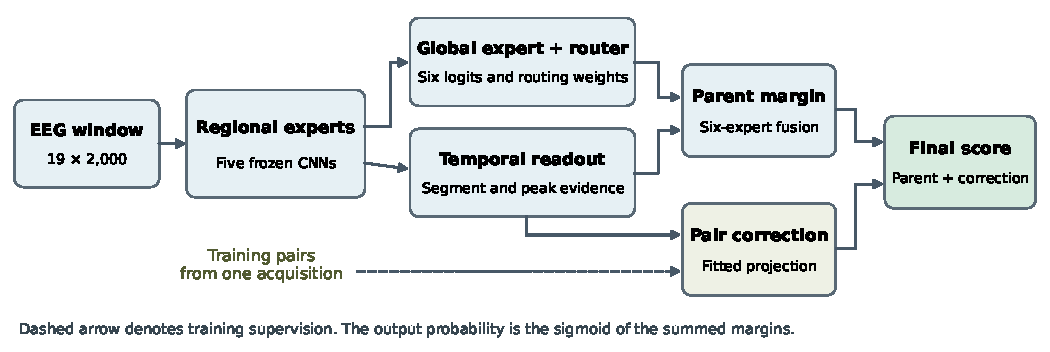
\includegraphics[width=0.94\textwidth]{architecture.pdf}
\caption{Six-expert prediction and the pair correction. The global expert takes the five regional representations as input. The temporal readout adjusts the experts' evidence before dense fusion. The correction projects a regional descriptor onto coefficients estimated from same-acquisition training pairs. The group and historical controls enter only during training.}\label{fig:architecture}
\end{figure*}

\subsection{Recovering temporal evidence}
The frozen encoders expose an activation sequence with 63 temporal positions. For each regional source we keep eight consecutive segment means of its projected activations before LayerNorm. The segments have lengths $(8,8,8,8,8,8,8,7)$. Let $b_{rj}$ denote the pre-normalization vector and $q_j$ its segment length divided by 63. The reference $\sum_j q_j b_{rj}$ therefore accounts for the shorter last segment. Giving it one eighth of the mass would introduce a difference even before learning any preference for a particular segment.

The regional frozen classifier maps each normalized segment to a margin, the positive logit minus the negative logit. A trainable scorer for each region takes the segment's feature deviation from $h_r$, its margin, the margin relative to the region's window score, and the mean segment margin across regions. A hidden layer with 32 units produces a scalar $s_{rj}$, bounded to $[-3,3]$ by a scaled hyperbolic tangent. In the arm studied here the weights are normalized separately for each expert:
\begin{equation}
  \alpha_{rj}=\frac{q_j\exp(s_{rj})}{\sum_k q_k\exp(s_{rk})}.
\end{equation}
The final scorer layers start at zero. Initially all regions pool with the same length-based reference, regardless of how strongly an individual segment activates a source classifier.

Let $N_r$ denote the source's projection normalization. The model adds the following shift to $h_r$:
\begin{equation}
  v_r=N_r\!\left(\sum_j\alpha_{rj} b_{rj}\right)
       -N_r\!\left(\sum_j q_j b_{rj}\right).
\end{equation}
The regional logit update is the difference between the frozen classifier applied to $h_r+v_r$ and to $h_r$. This construction uses each classifier in the feature coordinates on which it was trained. It also yields an exact zero update when pooling weights equal their reference. A small network takes all five feature shifts and changes in segment mass and predicts a global margin adjustment bounded in magnitude by 1.5.

The extended parent includes a separately supervised peak-shape readout. It uses activation maxima relative to mean and standard deviation, together with transformed location and scale features. This captures an aspect of within-window variation that can be lost in pooling. The final parent adds the router-weighted changes in the six expert logits to the peak-shape output. We use $m(x)$ to denote the resulting binary margin, immediately before the pair correction. All four memory variants share this parent design.

\subsection{Supervision and gradient paths}
The original core retains its training objective, including its task and global auxiliary terms. The additional components train on separate losses, with earlier branch outputs detached where they serve as references. The temporal allocation readout adds acquisition-weighted focal classification, a matched ranking term with coefficient 0.03 and a regional focal auxiliary term with coefficient 0.1 averaged over the five adjusted regional heads. The acquisition weights are computed from training-label frequencies within groups. The peak-shape and earlier readouts retain their own supervision.

This division matters for attribution. Even with an identical stream of examples, the expanded model can use a label to supervise more than one output. The parent also has additional capacity to represent evidence within each expert. A comparison between the final model and the original baseline includes these changes. The simultaneous parent output measured during each fit provides a more local comparison for the analytic pair correction.

\section{Within-Acquisition Pair Ranking}
\subsection{Descriptors and matched controls}
For each region the pair descriptor includes the first 32 coordinates of its frozen window representation and seven scalars. The first scalar is the adjusted regional window margin. The other six summarize the eight segment margins: their mean, population standard deviation, maximum, minimum, mean of the largest two values, and mean absolute change between adjacent segments. Concatenation gives $d(x)\in\mathbb{R}^{195}$. The last statistic distinguishes smoothly varying scores from scores that fluctuate across neighboring segments. Using six summaries keeps the matrix accumulated below small enough to solve repeatedly.

We derive acquisition groups from the training path hierarchy and retain groups with at least 50 training windows of each label for the pair estimator. Nine groups meet that condition. The full dataset still trains the parent. A FIFO ring holds up to 2,048 previously drawn eligible negatives across all groups. For a current eligible positive we filter the ring to its own group and order the remaining negatives by their collection-time mean adjusted regional margin. For $N$ available controls we take $K=\min(16,N)$ positions. Their zero-based sorted indices are $\lfloor(j+1/2)N/K\rfloor$, for $j=0,\ldots,K-1$.

Two details determine which labels can enter a comparison. First, negatives from the current batch are inserted only after its positives have been processed. If no earlier control meets the group criterion, that positive contributes no pair. Second, the ring is shared across groups. A group with more frequent negatives can occupy more slots, so matching does not equalize the number of comparisons supplied by different acquisitions. Group eligibility concerns unique manifest rows, whereas the pair counts we report concern sampled occurrences across epochs.

\subsection{A regularized margin update}
The parent produces a binary margin for each positive and negative. An online affine logistic calibration of this margin uses all sampled rows and maintains a slope $a$ and intercept. The intercept cancels in a pair difference. Given a positive and one selected negative, form the feature difference $u=d^+-d^-$ and margin gap $g=m^+-m^-$. Features are clipped coordinatewise to $[-32,32]$ before subtraction. Let $p=\sigma(\mathrm{clip}(ag,-12,12))$ be the estimated probability of ordering the pair correctly.

At zero feature correction the residual for the preferred ordering is $1-p$ and its logistic curvature is $p(1-p)$. For every comparison the implementation accumulates
\begin{align}
  H &\leftarrow H + p(1-p)uu^\top,\label{eq:gram}\\
  b &\leftarrow b + (1-p)u.\label{eq:rhs}
\end{align}
A pair with a strongly positive parent gap has a small residual. A pair ordered in the other direction contributes more to the right-hand side, scaled by its descriptor difference. These statistics retain evidence about which differences consistently accompany an under-ranked positive. The features and gaps are evaluated when the comparison occurs. Later changes in the parent do not retroactively change earlier terms in $H$ and $b$.

After at least four positives have formed pairs, the estimator solves
\begin{equation}
    (H+nD)w=b,\label{eq:solve}
\end{equation}
where $n$ is the number of comparisons. The diagonal of $D$ is the empirical variance of each descriptor coordinate over eligible training draws, floored at $10^{-4}$. The diagonal penalty scales with both the number of pairs and feature variability. The solver uses FP64 sufficient statistics. It checks for new comparisons every eight batches and can finalize a pending update on entry to evaluation. Each solve uses accumulated information from the observed stream. It does not require a second pass over training pairs.

At prediction time let $\mu$ be the mean clipped descriptor over eligible training observations. The correction to the margin is
\begin{equation}
 \delta(x)=\mathrm{clip}\!\left(
   \frac{2}{a}\tanh\!\left(\frac{(d(x)-\mu)^\top w}{2}\right),-6,6\right),
\end{equation}
with the same coordinatewise descriptor clipping understood. We add $\delta$ symmetrically to the two class logits as $(-\delta/2,+\delta/2)$. Until the ranker has collected sufficient comparisons, $\delta=0$. Once fitted, it needs only a descriptor from the current window and the saved coefficients and moments. No nearest-neighbor search, acquisition lookup or historical EEG is required to evaluate a new window.

\subsection{Which reference margins should be refreshed?}
The memory stores descriptors, a risk key and a scalar parent margin for each eligible negative. It also records the training row and epoch so that the original feature packet can be read again. During training a stored score can differ from the current parent's prediction because parameters have changed or because dropout was active. Replaying in evaluation mode removes the current dropout draw. Refreshing several controls augments the computation per eligible positive while preserving the optimizer step count.

Table~\ref{tab:arms} describes the four variants. When case refresh is enabled, eligible positives are re-scored before both the marginal calibration update and the pair comparisons. When control refresh is enabled, the model re-scores the union of selected slots in the batch and stores their new margins. Reuse of a control can therefore benefit the next comparison until eviction. The risk key and existing descriptor stay as collected. The full method calls the current parent in evaluation mode without gradients and restores its previous training modes afterward.





\section{Experimental Protocol}
\subsection{Data and sampling}
The input manifest contains 731,610 training windows (190,413 positive) and 166,079 validation windows (3,471 positive). The unit of prediction is one binary-labeled window. Training and validation contain different positive fractions, about 26.0\% and 2.09\%. In addition, the optimizer sees a sampled training distribution with only 645 positives in 20,000 draws per epoch. These three frequencies serve different purposes. The training manifest supplies the group-specific class counts used for matching, the validation class mix determines the operating characteristics on validation, and the sampled distribution determines how frequently the estimator encounters a positive in training.

The loader retains the first 19 channels in their stored order. It divides each input by $10^{-3}$ in its stored numeric precision, then copies up to 2,000 samples per channel into a zero-initialized FP32 buffer. The same preprocessing and five frozen source checkpoints are used throughout. The manifest provides validation recording folders but lacks a verified patient identifier. We retain the existing split for comparison with the historical protocol and separately examine the consequences of grouping by recording.

The baseline samples 19,355 negatives and 645 positives without replacement within each epoch. Repeated appearances in different epochs are possible. It uses 156 full batches of 128 windows and one final batch of 32. With 20 epochs, every fit has 400,000 training draws and 3,140 AdamW updates. The learning rate is $5\times10^{-4}$, weight decay is 0.01, and the focal parameters are $\alpha=0.85$ and $\gamma=2$. Both the training and evaluation batch sizes are 128. Training uses FP32 with a per-process GPU memory cap of 4 GiB. The analytic solver has its own FP64 buffers.

\subsection{Pairing and execution}
We compare each method at seeds 3 and 42. We check the frozen-file digests and the initialization hash for the trainable parameters shared with the original core. Two order checks are made per epoch: one records the sampled row indices, the other records their order after the batch sampler has been applied. All ten method--seed runs pass the formal configuration comparison and match the corresponding baseline sampler hashes for all 20 epochs. The original configuration permits nondeterministic GPU execution. An initialization or order match does not make independently trained arms bitwise-identical.

The candidate caches frozen features to avoid recomputing the five convolutional networks for every repeated draw. Extraction includes the special packets for the original partial batches. For the final comparison we re-ran the selected candidate checkpoints using all six experts on the raw validation windows. The largest absolute discrepancies from cached probabilities were $9.30\times10^{-5}$ and $6.72\times10^{-5}$ for seeds 3 and 42. Zero decisions changed at the two selected thresholds. This check addresses execution differences at the operating point used for the headline claim.

The strict baseline has 365,576 trainable parameters. The full model has 2,826,520, about 7.7 times as many, as well as the historical memory and analytic buffers. Additional head evaluations occur during score refresh. Matching the draw and optimizer budgets makes the comparison informative about reuse of the available examples. It does not match floating-point operations, elapsed training time or the number of times each representation is used in a supervised term.

\subsection{Endpoint and model selection}
We classify a window as positive when its score is strictly greater than the threshold. At each epoch we scan the 99 thresholds from 0.01 to 0.99 in steps of 0.01. We select the epoch and threshold that maximize positive-class window F1, $2\mathrm{TP}/(2\mathrm{TP}+\mathrm{FP}+\mathrm{FN})$, separately for every run. The reported mean averages the two seed-specific F1 values on the same validation windows. It is the performance summary of two training runs, with no prediction averaging across seeds. Average precision (AP) uses the complete ordering of scores and is reported separately.

The validation split was inspected during method development. We preserve this endpoint to answer the narrow question about improvement under the original selection protocol. To understand sensitivity we also select epochs by AP, inspect the parent and corrected heads within the same run, constrain the number of false positives, and select operating points with recording folds held out. These sensitivity analyses revisit the same source cohort. The four-hospital test below uses separate manifests.

\section{Results}
\subsection{The combined model and the refresh ablation}
The full method improves F1 over the strict baseline for each seed (Table~\ref{tab:main}). The mean increases from 69.787 to 72.032. The individual full-model results, 72.096 and 71.967, lie on opposite sides of 72. At the chosen checkpoints both models assign relatively high thresholds to their positive predictions, and the full model's selected threshold is 0.95 for both seeds. Threshold values cannot be compared as absolute measures of confidence across differently trained readouts.

\begin{table}[t]\centering\small
\caption{Validation F1 in percent. Each run uses its own selected epoch and grid threshold. Differences between scores in the text are percentage points.}\label{tab:main}
\begin{tabular}{lrrr}\toprule
Training method & Seed 3 & Seed 42 & Mean\\\midrule
Strict baseline & 69.390 & 70.184 & 69.787\\
Collection-time scores & 71.869 & 72.150 & 72.009\\
Refresh cases & 71.849 & 72.068 & 71.959\\
Refresh controls & 71.939 & 72.099 & 72.019\\
Refresh both & 72.096 & 71.967 & 72.032\\\bottomrule
\end{tabular}
\end{table}

Most of the separation from baseline is already present with scores evaluated at collection time. That variant gains 2.222 points on average, leaving 0.023 points between it and the full model. The largest and smallest two-seed means among the four memory policies are about 0.073 points apart. Refreshing both sides produces the highest score for seed 3, whereas retaining the original scores produces the highest score for seed 42. These observations give little basis for recommending the extra refresh computation solely on the strength of this validation result.

The eligibility criterion limits the number of observations that can distinguish these policies. The full-model fits encounter 138 and 150 eligible positive draws, compared with 12,900 total positive draws per fit. Each eligible positive in these runs finds 16 controls, yielding 2,208 and 2,400 pairs by the end of training. The 16 comparisons share the same positive window and some negatives can be selected more than once. Treating thousands of pairs as independent positive examples would exaggerate the evidence available to estimate a refresh effect.

\paragraph{Contribution of the pair correction within a run.}
At the full model's selected epoch, evaluating its temporal parent on the same windows with a separately selected grid threshold gives a direct comparison between two outputs of one fit. The corrected head gains 0.756 and 0.559 F1 points over that parent for seeds 3 and 42. Allowing each output to select its own best epoch reduces the differences to 0.433 and 0.262 points. At the parent's own best epoch, the corrected score instead trails by 0.311 and 0.353 points. Choosing the epoch from one of the two heads can favor the chosen head. Reporting all three comparisons makes this dependence visible.

Across the 20 epochs the corrected output exceeds its simultaneous parent's F1 in 18 epochs for seed 3 and 13 for seed 42. These checkpoints are successive states of a single training process. Their signs describe the trajectory and cannot be counted as independent replications. The size of the within-run correction is smaller than the full-model gain over the strict baseline. Separating the remaining gain among temporal allocation, peak-shape features, parameter count and auxiliary supervision would require additional paired controls.

\subsection{What happens to individual decisions?}
Table~\ref{tab:episodes} gives the operating points underlying the F1 scores. For seed 3 recall rises by 6.68 points and precision falls by 1.94 points. For seed 42 recall rises by 4.06 points and precision falls by 0.81 points. The accuracy of both models rounds to approximately 99\%, reflecting the dominance of negative windows. Counts and class-specific rates show the trade-off more directly.

\begin{table*}[t]\centering\small
\caption{Raw-input operating points at the validation-F1-selected checkpoints. P, R, AP and AUROC are percentages. AP and AUROC use the score ordering across all validation windows.}\label{tab:episodes}
\begin{tabular}{llrrrrrrrrrr}\toprule
Seed & Model & Epoch & Threshold & TP & FP & FN & TN & P & R & AP & AUROC\\\midrule
3 & Baseline & 2 & 0.81 & 2,251 & 766 & 1,220 & 161,842 & 74.61 & 64.85 & 75.25 & 97.72\\
3 & Full & 5 & 0.95 & 2,483 & 934 & 988 & 161,674 & 72.67 & 71.54 & 74.73 & 98.45\\
42 & Baseline & 5 & 0.82 & 2,321 & 822 & 1,150 & 161,786 & 73.85 & 66.87 & 75.68 & 97.82\\
42 & Full & 4 & 0.95 & 2,462 & 909 & 1,009 & 161,699 & 73.03 & 70.93 & 75.61 & 98.43\\\bottomrule
\end{tabular}
\end{table*}

Net counts can hide changes in both directions. We joined the two decision vectors in validation order, checking label equality before the comparison. For seed 3 the two models agree on 2,219 positive windows that they detect and 956 that they miss. The full model recovers 264 additional positives while losing 32 detected by the baseline. On negative windows it adds 274 false positives and removes 106. The corresponding seed-42 changes are 225 positives recovered and 84 lost, with 281 new false positives and 194 removed. Thus the larger recall gain for seed 3 reflects both more recoveries and fewer losses among baseline detections.

\paragraph{A fixed false-positive budget.}
To distinguish a change in ranking from a willingness to issue more alerts, we keep the selected checkpoints and examine every threshold on the original grid. For each seed we take the lowest full-model threshold whose number of false positives is at most the baseline count. We evaluate that threshold on the same validation windows. This is a retrospective operating-point analysis, with no refit or interpolation between grid thresholds.

For seed 3 the baseline budget is 766 false positives. At 0.96 the full model still produces 814, so the first feasible grid point is 0.97. It detects 2,279 positives and flags 670 negatives, gaining 28 true positives while using 96 fewer false positives than the baseline. For seed 42 the first feasible threshold is 0.96, giving 2,338 true positives and 725 false positives against a budget of 822. The gain in detections is 17 with 97 fewer false positives. At these thresholds the full model's F1 is 71.00 and 71.56. The 72.032 mean describes a more permissive operating point. Most of the gain in detections at that point is coupled to a higher alert count.



The difference in the spacing of points in Figure~\ref{fig:budget} is consequential. For seed 3, moving the full model from 0.95 to 0.97 removes 264 false positives but also loses 204 true positives. A common numeric threshold for both models would mix differences in score scale with differences in ordering. A common count budget makes the desired error constraint explicit. The grid leaves some of that budget unused in both seeds, so this calculation is conservative about attainable recall between adjacent grid values.

\subsection{Dependence on the checkpoint criterion}
Figure~\ref{fig:curve} follows the best grid F1 at each epoch. A comparison at the same epoch favors the full model over the strict baseline in all 20 epochs for each seed. Median same-epoch gains are 2.03 and 2.57 points, respectively. The final-epoch scores are 69.80 and 70.93 for the full model, compared with 68.46 and 68.65 for baseline. Consequently, the direction of the paired difference persists at the end of training even though the 72-point mean depends on selecting an earlier checkpoint.



AP answers a different question about the same scores. At the F1-selected epoch the full model has slightly lower AP for both seeds, despite higher AUROC and F1. If we choose the epoch by AP instead, the peak AP values for seed 3 are 75.53\% for baseline and 77.87\% for the full model. The corresponding values for seed 42 are 75.76\% and 77.28\%. Evaluating grid F1 at those AP-selected checkpoints gives 69.27 versus 71.46 and 70.15 versus 71.59. This comparison still uses validation to select the threshold, but shows how the conclusion about crossing a particular F1 target depends on which statistic selects the weights.

\section{Sensitivity to the Recording Split}
\subsection{Selection with recordings held out}
Windows with nearby or related recordings may share properties. A bootstrap that draws windows independently would neglect that structure. We use the 72 full validation recording directories as grouping units and sample that many directories with replacement, counting all their windows. Baseline and candidate receive the same draw. Across 3,000 draws the central 95\% intervals for the F1 difference are $[0.972,5.319]$ and $[0.167,4.234]$ points. These intervals condition on the selected checkpoints and thresholds. They describe variability across these recording groups, and exclude uncertainty from training, architecture selection or transfer to new patients.

To probe operating-point selection, we further partition the validation set into five stratified folds grouped by full recording directory. For each fold and each fit, we select both the epoch and the threshold on the other four folds. We then evaluate the held-out folder predictions at that choice and pool their confusion counts. The pooled F1 weights windows through the confusion counts and is generally different from the arithmetic mean of five fold F1s. No model is retrained in this exercise. All learned checkpoints and the choice of architecture already existed.

\begin{table}[t]\centering\small
\caption{F1 under alternative choices of windows and operating points. Each entry is baseline / full model. The exclusion keeps the primary thresholds fixed.}\label{tab:transfer}
\begin{tabular}{lcc}\toprule
Comparison & Seed 3 & Seed 42\\\midrule
All validation windows & 69.39 / 72.10 & 70.18 / 71.97\\
Recording-fold selection & 68.27 / 72.10 & 69.80 / 70.29\\
Exclude shared names & 67.00 / 70.30 & 67.98 / 70.13\\\bottomrule
\end{tabular}
\end{table}

For seed 3 the full model selects epoch 5 and threshold 0.95 on every four-fold selection subset. Its held-fold predictions therefore reproduce the primary result exactly. Seed 42 selects epoch 4 or 5 for four folds and epoch 18 for the fifth. The corresponding grid thresholds span 0.89 to 0.97. Its pooled held-fold F1 drops to 70.29, about half a point above the corresponding baseline (Table~\ref{tab:transfer}). Looking at the counts explains the reduction: the pooled full-model predictions contain 2,463 true positives and 1,074 false positives, compared with 2,462 and 909 in the primary analysis. Nearly all the change is on negative windows.

The pooled results conceal considerable differences between folds. For seed 3 the full model's advantage ranges from 1.33 to 7.10 points, with the largest gain on the fold where the baseline performs worst. For seed 42 all five held-fold differences are positive, but the smallest is only 0.014 points and the largest is 1.24. Both seeds use exactly the same recording partition. The contrasting gain ranges illustrate sensitivity to the trained model and its selected operating point as well as to the recording mix. Five overlapping selection subsets cannot establish a distribution of effects over independent cohorts. The appendix gives their selected operating points.

\paragraph{Transferring the false-positive budget.}
Using the same fold-specific epochs, we also matched the full model to the baseline false-positive count on the four selection folds. We then applied both thresholds to the held recordings. Across all held windows, seed 3 gained 110 true positives and issued 107 fewer false positives (F1 71.50 versus 68.27). Seed 42 lost 16 true positives and issued 113 fewer false positives (70.69 versus 69.80). The full model exceeded the baseline's false-positive count on two held folds for seed 3 and one for seed 42. Meeting a budget on the selection recordings thus gave neither a per-fold guarantee nor a consistent recall gain on held recordings.

\subsection{A proxy for cross-split identity}
The manifest contains ten repeated file-path rows and no exact training--validation path overlap. Three recording-directory basenames occur in both splits. A repeated basename can correspond to the same person, a reused naming convention or a different recording. Conversely, a person may appear under multiple names. We can test the effect of excluding these names while keeping the limits of this proxy explicit.

The exclusion removes 2,582 validation windows, including 394 positives. These windows account for about 1.55\% of validation windows but 11.35\% of its positives. Holding the original thresholds and epochs fixed gives full-model F1 of 70.30 and 70.13 on the retained windows. The paired gains over baseline are 3.30 and 2.15 points. The absolute scores drop and the paired gains remain positive. Because F1 depends on class prevalence and because this subset can differ in difficulty, that drop alone cannot quantify leakage. Within the removed subset itself, the full model gains 12 and 6 true positives while adding 29 and 14 false positives. On the retained subset it gains 220 and 135 true positives, accounting for most of the net increase in detections. This decomposition is possible with fixed operating points because TP and FP counts add across disjoint sets. F1 is nonlinear, so analogous subtraction of two F1 scores does not identify the contribution of the excluded recordings. Verifying patient identity would require information outside the manifest.

\section{Transfer to Four External Hospitals}
We evaluated all binary-labeled test windows supplied by Qilu, Tiantan, Chifeng and Xi'an (698,502 windows total). For each seed we locked the original Xiehe-selected checkpoint and threshold before external inference. All four sites used identical channel ordering, input scaling and window length. The model saw neither the hospital identifier nor its labels at prediction time. We used each hospital's labels only to evaluate the resulting scores. The mean for a hospital is the arithmetic mean of its two seed-specific window F1s.
\begin{table}[t]\centering\small
\caption{External positive-class window F1 (percent), averaged over seeds 3 and 42 at the source-selected thresholds. Each hospital contributes one value to the last row.}\label{tab:external}
\begin{tabular}{lrrr}\toprule
Hospital & Baseline & Full model & Difference\\\midrule
Qilu & 61.89 & 63.77 & +1.88\\
Tiantan & 42.37 & 41.57 & -0.80\\
Chifeng & 42.22 & 45.73 & +3.51\\
Xi'an & 24.19 & 31.44 & +7.25\\
\midrule
Equal-site mean & 42.67 & 45.63 & +2.96\\\bottomrule
\end{tabular}
\end{table}

The full model improves F1 for both seeds at Qilu, Chifeng and Xi'an, while both seeds decline at Tiantan (Table~\ref{tab:external}). The equal-site mean rises from 42.67 to 45.63. Xi'an has the largest gain, 7.25 points, yet full-model recall there averages only 21.13\%. At Tiantan the model finds 136 and 37 more true positives but adds 679 and 555 false positives, respectively. Mean recall rises from 73.57\% to 75.59\%, while precision falls from 29.75\% to 28.67\%. Transporting the source operating point therefore changes the balance of errors in a site-dependent manner. Per-seed counts and ranking metrics are in the appendix.

\section{Discussion and Conclusion}
The experiments distinguish three decisions. Adding the entire temporal and pair-based readout increases F1 across both seeds. Applying the fitted pair correction to its immediate parent produces a smaller gain that depends on which head selects the checkpoint. Recomputing stale margins for that correction changes mean F1 by only 0.023 points and has opposite effects by seed. If training compute is constrained, collection-time scoring is already competitive on the observed data. The present comparisons do not determine whether the same choice would be best for a stream with more eligible positive windows or a faster-changing parent.

For an application with a false-alert constraint, the decision budget is as important as the architecture. At the primary operating points the full model adds 232 and 141 true positives. Within the strict baseline's false-positive budget on the same grid, the increases are 28 and 17. Both observations matter: the six-source readout improves the trade-off locally, and the headline recall gains are larger than the gains achievable at the original false-positive count. A window flagged twice in one episode could contribute two false positives here, so none of these counts is a rate of alerts per recording hour or per patient.

The principal limitations are repeated selection on one development split, two training seeds, unequal model capacity and unverified patient identities. A prospective follow-up would verify patient identities and lock the target definition and alert policy before collecting data. A parameter- and compute-matched temporal parent trained without pair supervision would answer a different question: how much of the observed improvement can be purchased by capacity and additional supervised readouts alone? The two-seed F1 is 72.032 on the source validation set and 45.63 when each of the four external hospitals is weighted equally. The difference between these endpoints is central to interpreting the source result.

\clearpage
\section*{Impact Statement}
The model classifies individual EEG windows. The observed gains in sensitivity are accompanied by extra false positives at the F1-selected thresholds. Using these results to guide clinical decisions would require a clinically validated target definition, patient-level evaluation and an assessment of the consequences of alerting on consecutive windows. The release provides aggregate validation statistics and code. Recording identifiers and waveforms remain with the data custodians.

\section*{AI Disclosure Statement}
An OpenAI coding assistant helped examine the implementation and run records, locate literature, draft the manuscript, generate figures and package the reproducibility material. The decision-overlap and threshold-budget analyses use stored validation predictions. External and expert-activity tables summarize model outputs on the original manifests. This public preprint awaits independent review by the project authors.

\bibliography{references}
\bibliographystyle{icml2026}

\clearpage
\appendix
\onecolumn
\section{Reproducing the Tables}
The released selected-checkpoint table contains the threshold, epoch, confusion matrix, AP and AUROC for each method and seed. The epoch table covers all 200 method--seed--epoch combinations. F1 is calculated from integer counts before conversion to percentages. The public verifier needs the Python standard library to check the counts, epoch-level selection, sampler agreement and source digests.

The public operating-point file contains the two sets of 99 raw-input confusion-count pairs per seed and the decision-overlap counts at the selected thresholds. The accompanying script checks raw prediction files against the previously released counts before exporting these aggregates. The false-positive-budget comparison chooses the first feasible threshold in increasing grid order. Its counts can be recovered directly from the public file. Recreating per-window predictions requires authorized access to the original EEG, manifest and regional checkpoints.

\begin{table}[h]\centering\small
\caption{At the primary operating points, the number of windows that each model flags, by true label. All counts refer to the same 166,079 windows in each seed.}\label{tab:appendoverlap}
\begin{tabular}{llrrrr}\toprule
Seed & True label & Both & Base only & Full only & Neither\\\midrule
3 & Positive & 2,219 & 32 & 264 & 956\\
3 & Negative & 660 & 106 & 274 & 161,568\\
42 & Positive & 2,237 & 84 & 225 & 925\\
42 & Negative & 628 & 194 & 281 & 161,505\\\bottomrule
\end{tabular}
\end{table}

The recording-fold analysis selects the first threshold tying for maximum F1 at a given epoch and the last epoch tying for maximum F1 across epochs. Each validation window contributes to exactly one held-fold confusion matrix. The folder bootstrap instead keeps one epoch and threshold per model fixed throughout the resamples. The false-positive-budget transfer uses the same fold-specific epochs and baseline operating points, then selects the lowest full-model grid threshold that satisfies the baseline count on the four selection folds. Fold-level selection and held counts for that analysis accompany the public results.
\begin{table}[h]\centering\small
\caption{Operating points transferred across validation recording folds. Each entry gives the epoch, threshold and held-fold F1 (percent). Each model chooses its operating point using the other four folds.}\label{tab:folds}
\begin{tabular}{lcccc}\toprule
& \multicolumn{2}{c}{Seed 3} & \multicolumn{2}{c}{Seed 42} \\
Fold & Baseline & Full & Baseline & Full \\\midrule
1 & 3 / 0.80 / 58.49 & 5 / 0.95 / 65.60 & 7 / 0.82 / 60.37 & 18 / 0.89 / 61.23 \\
2 & 2 / 0.81 / 71.30 & 5 / 0.95 / 73.68 & 5 / 0.82 / 72.69 & 5 / 0.97 / 72.70 \\
3 & 2 / 0.80 / 69.41 & 5 / 0.95 / 70.74 & 5 / 0.82 / 70.18 & 4 / 0.95 / 70.55 \\
4 & 2 / 0.81 / 70.52 & 5 / 0.95 / 73.20 & 5 / 0.82 / 70.68 & 5 / 0.97 / 71.92 \\
5 & 7 / 0.82 / 72.72 & 5 / 0.95 / 76.45 & 5 / 0.82 / 74.68 & 4 / 0.95 / 75.48 \\
\bottomrule\end{tabular}
\end{table}

\clearpage
\section{Model and Operating-Point Diagnostics}
Algorithm~\ref{alg:update} describes the full training step. The descriptors and risk key of a negative retain their collection-time values. Only the selected negative's scalar parent margin is overwritten when it is refreshed. Table~\ref{tab:arms} identifies which inputs change in each separately trained arm.
\begin{table}[htbp]\centering\small
\caption{Source of the scalar margins when a pair is formed. Each arm is trained from the same shared initialization for a given seed.}\label{tab:arms}
\begin{tabular}{lll}\toprule
Arm & Positive margin & Negative margin\\\midrule
Collection time & As collected & As collected\\
Refresh cases & Current parent & As collected\\
Refresh controls & As collected & Current parent\\
Refresh both & Current parent & Current parent\\\bottomrule
\end{tabular}
\end{table}
\begin{algorithm}[htbp]
\caption{One training batch in the full method}\label{alg:update}
\begin{algorithmic}[1]
\STATE Compute parent outputs and descriptors for the batch.
\FOR{each eligible positive in the batch}
  \STATE Select prior same-group controls at risk quantiles.
\ENDFOR
\STATE Re-score eligible cases and selected control slots with the current evaluation-mode parent.
\STATE Update the calibration statistics using the batch.
\FOR{each selected case--control pair}
  \STATE Accumulate its contributions to $H,b$ in Eqs.~\ref{eq:gram}--\ref{eq:rhs}.
\ENDFOR
\STATE Insert the batch's eligible negatives into the ring.
\STATE Update coefficients when due using Eq.~\ref{eq:solve}.
\STATE Apply the scheduled parent optimizer update.
\end{algorithmic}
\end{algorithm}
\paragraph{Budget transfer and checkpoint selection.}
Figure~\ref{fig:budget} uses the source-validation selected checkpoints. The dotted line fixes the number of false-positive windows at each baseline's operating point. For comparison, the recording-fold budget analysis selects operating points on other recordings, and allows a held fold to exceed its selection budget. Figure~\ref{fig:curve} gives the complete F1 trajectories behind checkpoint selection.
\begin{figure}[htbp]\centering
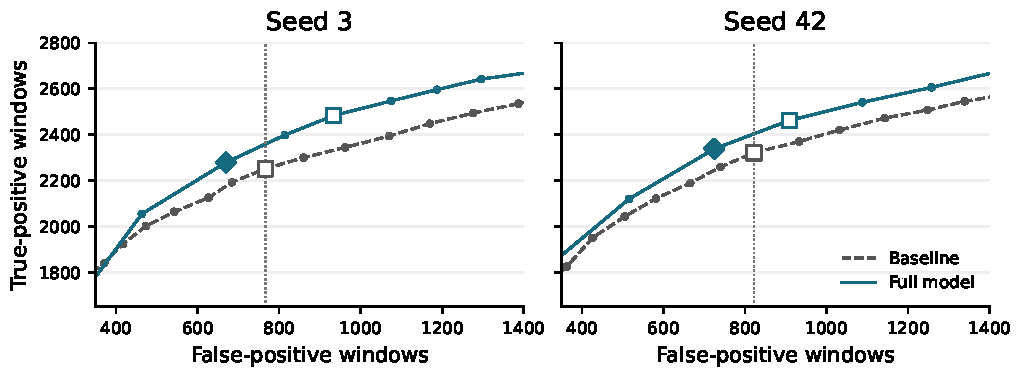
\includegraphics[width=0.90\textwidth]{operating_points.pdf}
\caption{True positives attainable at the original threshold grid near the two chosen operating points. Dots are grid points, squares mark each model's F1-selected threshold, and the vertical line is the baseline false-positive count. The diamond is the full model's lowest grid threshold satisfying that budget. Connecting lines guide the eye. Only the marked grid points enter the analysis.}\label{fig:budget}
\end{figure}
\begin{figure}[htbp]\centering
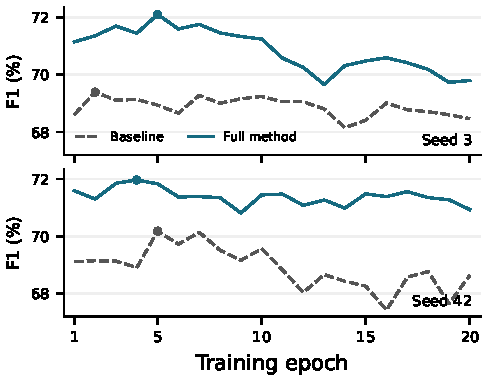
\includegraphics[width=0.54\textwidth]{epoch_f1.pdf}
\caption{Best validation-grid F1 at each epoch. Dots mark the checkpoints used in the primary comparison. Each trace covers one training run.}\label{fig:curve}
\end{figure}
\section{External Test Protocol and Per-Seed Results}
Each site manifest contained both target classes. We used every manifest row in its original order. Native batches contain 128 windows with a possible shorter last batch. The five frozen expert files were verified against the metadata of each of the four fitted models. The four fits share the same five convolutional backbones. During evaluation their last feature maps were computed once per batch, and each fit applied its own hooks, classification heads, router and fitted readout. A direct comparison recomputed the complete convolutional forward path on the first batch of every site partition and each partial final batch. It checked the final score, six routing weights and six expert scores against the shared-feature implementation.
The direct checks covered 4,486 windows in total with zero difference in every checked output. The positive/total window counts were 4,946/106,983 for Qilu, 4,283/325,755 for Tiantan, 440/46,053 for Chifeng, 504/219,711 for Xi'an. Specificity and true-negative counts are available in the accompanying CSV.
\begin{table}[htbp]\centering\small
\caption{All four held-site operating points per hospital. P, R, F1, AP, and AUROC are percentages. The original thresholds for baseline are 0.81/0.82 for seeds 3/42. The full model uses 0.95 for both.}\label{tab:externaldetail}
\begin{tabular}{lllrrrrrrrr}\toprule
Site & Model & Seed & TP & FP & FN & P & R & F1 & AP & AUROC\\\midrule
Qilu & Baseline & 3 & 3,073 & 1,979 & 1,873 & 60.83 & 62.13 & 61.47 & 58.22 & 92.91\\
Qilu & Baseline & 42 & 3,178 & 2,076 & 1,768 & 60.49 & 64.25 & 62.31 & 57.95 & 92.90\\
Qilu & Full & 3 & 3,244 & 1,940 & 1,702 & 62.58 & 65.59 & 64.05 & 63.68 & 93.90\\
Qilu & Full & 42 & 3,208 & 1,950 & 1,738 & 62.19 & 64.86 & 63.50 & 62.27 & 93.72\\
\midrule
Tiantan & Baseline & 3 & 3,092 & 7,309 & 1,191 & 29.73 & 72.19 & 42.11 & 27.73 & 97.20\\
Tiantan & Baseline & 42 & 3,210 & 7,570 & 1,073 & 29.78 & 74.95 & 42.62 & 27.64 & 97.21\\
Tiantan & Full & 3 & 3,228 & 7,988 & 1,055 & 28.78 & 75.37 & 41.65 & 25.31 & 97.40\\
Tiantan & Full & 42 & 3,247 & 8,125 & 1,036 & 28.55 & 75.81 & 41.48 & 25.28 & 97.38\\
\midrule
Chifeng & Baseline & 3 & 145 & 114 & 295 & 55.98 & 32.95 & 41.49 & 39.46 & 93.16\\
Chifeng & Baseline & 42 & 160 & 145 & 280 & 52.46 & 36.36 & 42.95 & 40.68 & 93.67\\
Chifeng & Full & 3 & 159 & 123 & 281 & 56.38 & 36.14 & 44.04 & 44.48 & 94.71\\
Chifeng & Full & 42 & 179 & 136 & 261 & 56.83 & 40.68 & 47.42 & 45.57 & 94.59\\
\midrule
Xi'an & Baseline & 3 & 72 & 40 & 432 & 64.29 & 14.29 & 23.38 & 19.08 & 71.52\\
Xi'an & Baseline & 42 & 78 & 42 & 426 & 65.00 & 15.48 & 25.00 & 19.88 & 72.57\\
Xi'an & Full & 3 & 105 & 61 & 399 & 63.25 & 20.83 & 31.34 & 24.06 & 78.27\\
Xi'an & Full & 42 & 108 & 73 & 396 & 59.67 & 21.43 & 31.53 & 23.92 & 76.16\\
\bottomrule\end{tabular}
\end{table}

\clearpage
\section{How the Six Experts Respond}
\label{sec:activity}
For each window we recorded the six dense routing weights and the six expert outputs before the final pair correction. We call the routing weight the expert's activation for this analysis. The weights sum to one across experts on a window. The positive-class expert score is the two-logit softmax output of one expert. Each expert has its own class distribution, so these six scores need not sum to one. The complete classifier also uses temporal and pair corrections. Neither a high weight nor a high score measures the causal importance of a brain region.

Figures~\ref{fig:expertweights} and~\ref{fig:expertscores} group windows by true label, site and seed, keeping the two seeds separate. Each cell is a mean over all windows in that stratum. A negative-heavy hospital therefore cannot mask how an expert responds to its rarer positive windows. Figure~\ref{fig:expertdist} displays the median and interquartile range for each individual expert on positive windows. These intervals describe variation across windows, not uncertainty in a population mean. The accompanying aggregate file also contains the strict baseline, the denominator of each group, and the number of windows in which each expert had the largest weight.
Averaged equally across seeds, the global and occipital experts together receive 89--91\% of the routing weight on negative windows at each site. Positive windows show larger differences. The frontal expert's mean positive-window weight ranges from 25.27\% at Xiehe to 6.55\% at Xi'an, where the global and occipital weights are 55.58\% and 29.41\%. The global expert's mean positive-class score on true positives is also lower at Xi'an (45.63\%) than at Xiehe (86.80\%). These are descriptive patterns in observed windows. The six sources each receive all 19 channels, and the figures alone cannot distinguish physiology, acquisition differences or label composition as explanations.

\begin{figure}[htbp]\centering
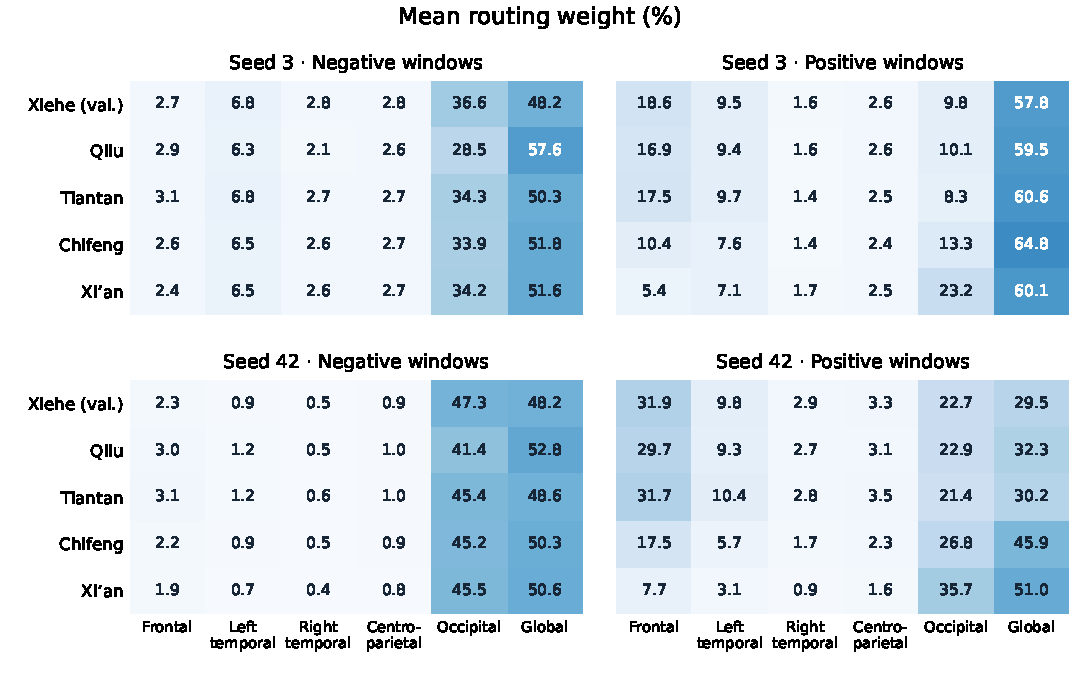
\includegraphics[width=.90\textwidth]{expert_routing.pdf}
\caption{Class-conditional mean routing weights of the full model. Each row sums to 100\% before rounding. Xiehe is the source validation set. The remaining rows are the external hospitals.}\label{fig:expertweights}
\end{figure}
\begin{figure}[htbp]\centering
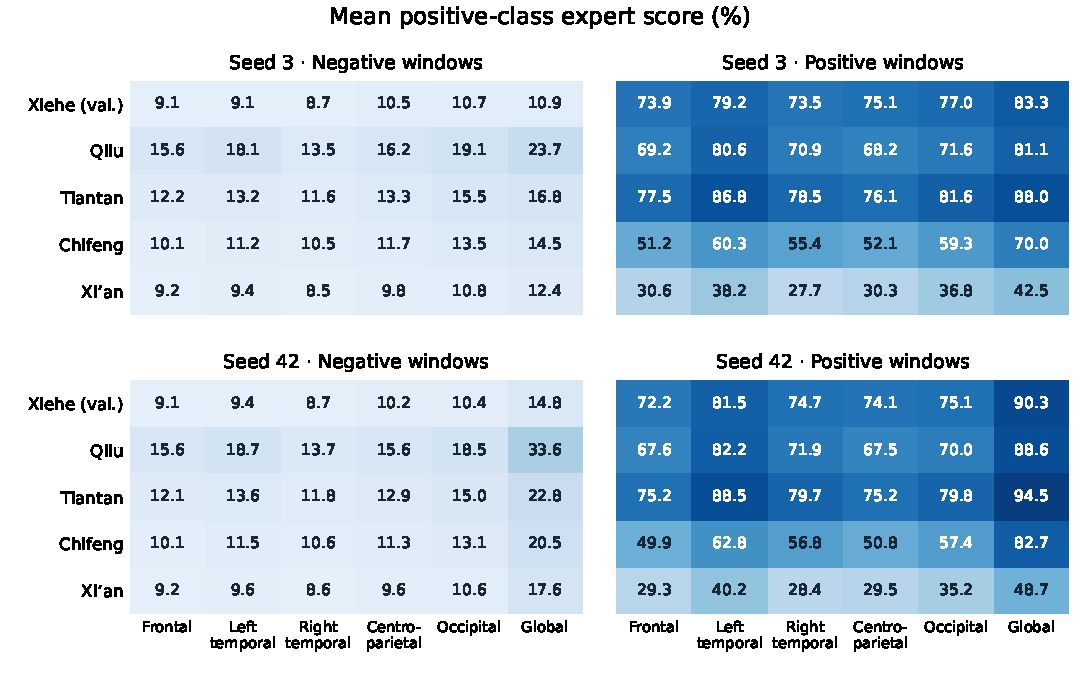
\includegraphics[width=.90\textwidth]{expert_scores.pdf}
\caption{Class-conditional mean positive-class score of each expert. A high score on true positives can coexist with a high score on negatives. Values are percentages.}\label{fig:expertscores}
\end{figure}
\begin{figure}[htbp]\centering
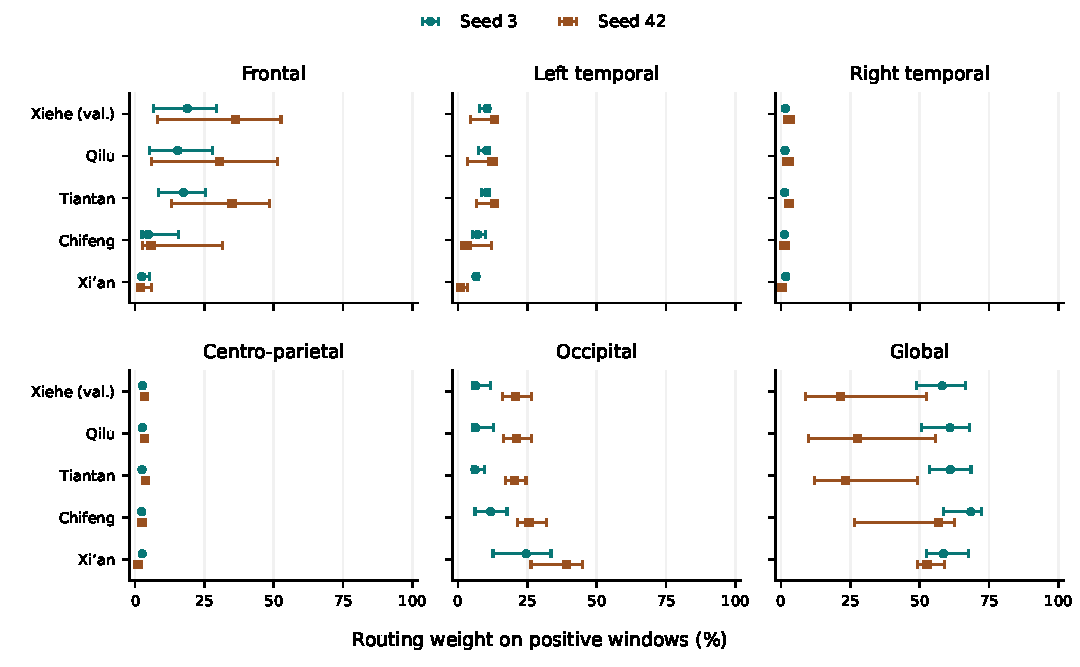
\includegraphics[width=.90\textwidth]{expert_distributions.pdf}
\caption{Routing-weight distributions for the six experts on true positive-class windows, including those the model misses. Points mark medians and whiskers span the 25th to 75th percentiles. The horizontal scale is shared across all panels.}\label{fig:expertdist}
\end{figure}
\end{document}
